\documentclass[lang=cn,blue]{elegantbook}
\title{模拟旅行查询系统}
\subtitle{课程实践报告}

\author{王嘉茜·于海鑫·田静悦}
\institute{北京邮电大学计算机学院}
\date{\today}

\version{1.00}
\logo{logo.png}
\cover{cover.jpg}

\usepackage{algorithm}
\usepackage{algpseudocode}
\usepackage{listings}
\newfontfamily\courier{Courier New}
\lstset{linewidth=1.1\textwidth,
	numbers=left,
	basicstyle=\small\courier,
	numberstyle=\tiny\courier,
	keywordstyle=\color{blue}\courier,
	commentstyle=\it\color[cmyk]{1,0,1,0}\courier, 
	stringstyle=\it\color[RGB]{128,0,0}\courier,
	frame=single,
	breaklines,
	extendedchars=false, 
	xleftmargin=2em,xrightmargin=2em, aboveskip=1em,
	tabsize=4, 
	showspaces=false
	basicstyle=\small\courier
}

\begin{document}
\maketitle
\tableofcontents
\mainmatter
\hypersetup{pageanchor=true}

\chapter{概述}
\section{任务描述}
任务要求建立一个旅客管理系统,该系统中内置了一张城市图表,旅客可以通过三种交通工具(汽车、火车、飞机)在各个城市间进行转移。用户(乘客)可以在任意时间对系统提出请求,系统应根据用户的输入为其确定一条旅游线路并输出。系统能模拟出旅客在旅行时某一时间内所处的地点和状态,并以日志的形式记录下来。用户输入应包括起点、终点、必经城市以及旅行策略。旅行策略共有如下三种:
\begin{enumerate}
	\item 花费最少策略
	\item 时间最少策略
	\item 限时花费最少策略
\end{enumerate}
\section{功能需求}
\begin{itemize}
	\item 城市总数不少于10个
	\item 建立汽车、火车和飞机的时刻表(航班表)
	\begin{enumerate}
		\item 有沿途到站及票价信息
		\item 不能太简单(不能总只是1班车次相连)
	\end{enumerate}
	\item 旅客的要求包括:起点、终点、途经某些城市和旅行策略
	
	旅行策略有:
	\begin{enumerate}
		\item 最少费用策略:无时间限制,费用最少即可
		\item 最少时间策略:无费用限制,时间最少即可
		\item 限时最少费用策略:在规定的时间内所需费用最省
	\end{enumerate}
	\item 旅行模拟查询系统以时间为轴向前推移,每10秒左右向前推进1个小时(非查询状态       的请求不计时);
	\item 不考虑城市内换乘交通工具所需时间
	\item 系统时间精确到小时
	\item 建立日志文件,对旅客状态变化和键入等信息进行记录
	\item 用图形绘制地图,并在地图上反映出旅客的旅行过程
\end{itemize}

\section{模型简化}
通过一些假设,我们可以剔除实际模型中不必要的变量,保留问题的本质和研究重点,简化模型。在这次课程实践中,我们提出了如下假设:
\begin{enumerate}
	\item 截至 2017 年,我国共有约 2000 个火车站办理客运业务,同时有约 220 个民用机场,汽车站更是不计其数。将这些场地全部添加到我们的系统内是不现实的,为了简化获取数据的难度,同时使最后的图形化界面更加简洁,我们只选取了除去港澳台外的全国 31 个行政区的省会城市进行建模。
	\item 可以注意到,对于火车来说,分段购票与直接购票的价格差较小(通常不超过票价的 10\%),因此我们可以假设只有相邻省份之间的城市拥有直达列车,并以沿途火车票价之和模拟不相邻省份之间的列车价格。
	\item 汽车不适用于远程交通,且其运输市场受路况等客观因素影响较大,难以精确求出其运行时间。我们假设只有相邻省份之间的城市可以通过汽车到达,且汽车的时间表是固定的。
\end{enumerate}

\section{解决方案说明}
在这一节内,我们对该系统使用的技术以及人员分工进行描述。
\subsection{编程语言}
该系统主体部分使用 C++ 进行开发,图形部分采用 Qt 框架以实现跨平台特性。爬虫部分使用 Python 的 requests 库进行开发。
\subsection{人员分工}
\begin{itemize}
	\item \textbf{于海鑫}\ 算法实现以及爬虫部分
	\item \textbf{王嘉茜}\ 图形界面
	\item \textbf{田静悦}\ 日志模块
\end{itemize}
\subsection{编程规范}
\begin{itemize}
	\item \textbf{C++}部分遵循 \href{http://www.nscscc.org/uploads/soft/170318/1-1F31P20H9.docxhttp://google.github.io/styleguide/cppguide}{Google C++ Style Guide}, 通过使用 clang 提供的工具包保证代码风格的一致性
	\item \textbf{Python}部分遵循 \href{https://www.python.org/dev/peps/pep-0008/}{PEP-8},使用 IDE 提供的检测功能保证代码风格的规范性
\end{itemize}
\vspace*{3 ex}
以下将分章介绍实现细节。

\chapter{总体设计}

该程序主体部分主要分为算法,图形界面,中间层三个模块。爬虫部分分为两个模块,分别处理来自于 12306 以及携程网的数据。因为爬虫部分过于简单,在此仅仅介绍主体部分的设计,以下是详细介绍。

主体部分的包含关系见图~\ref{main_cpp}~。其中的 \textbf{main.cpp} 是程序的入口点,Qt 的初始化以及文件的载入都在此处进行;\textbf{graph\_handler.h} 以及与之对应的 .cpp 文件则是算法层与图形界面的交互层,在这里算法层提供的接口被包装为 QML 可以调用的函数以及 Qt 的信号和槽;\textbf{city\_graph.h} 以及与之对应的 .cpp 文件是算法部分,在这里实现了三种策略的算法。

\begin{figure}[!htbp]
	\centering
	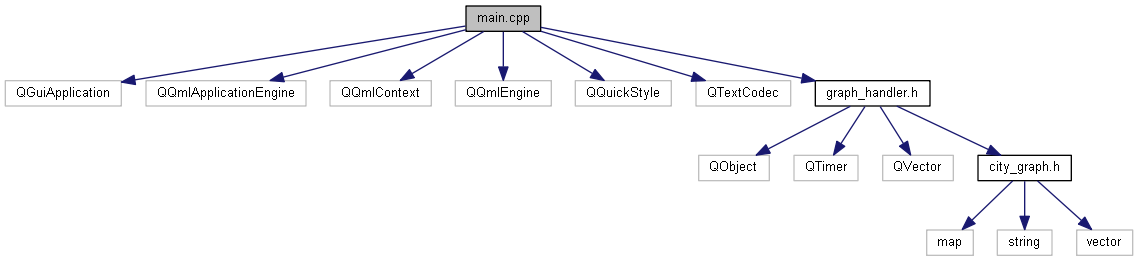
\includegraphics[width=1\textwidth]{main_8cpp__incl.png}
	\caption{主体部分的包含关系}
	\label{main_cpp}
\end{figure}

中间层对于算法部分的调用除了基本的设置各种初始值外,均集中于 \textbf{GraphHandler::generateResult} 函数内,该函数的调用图见图~\ref{genR}~。

 \begin{figure}[!htbp]
 	\centering
 	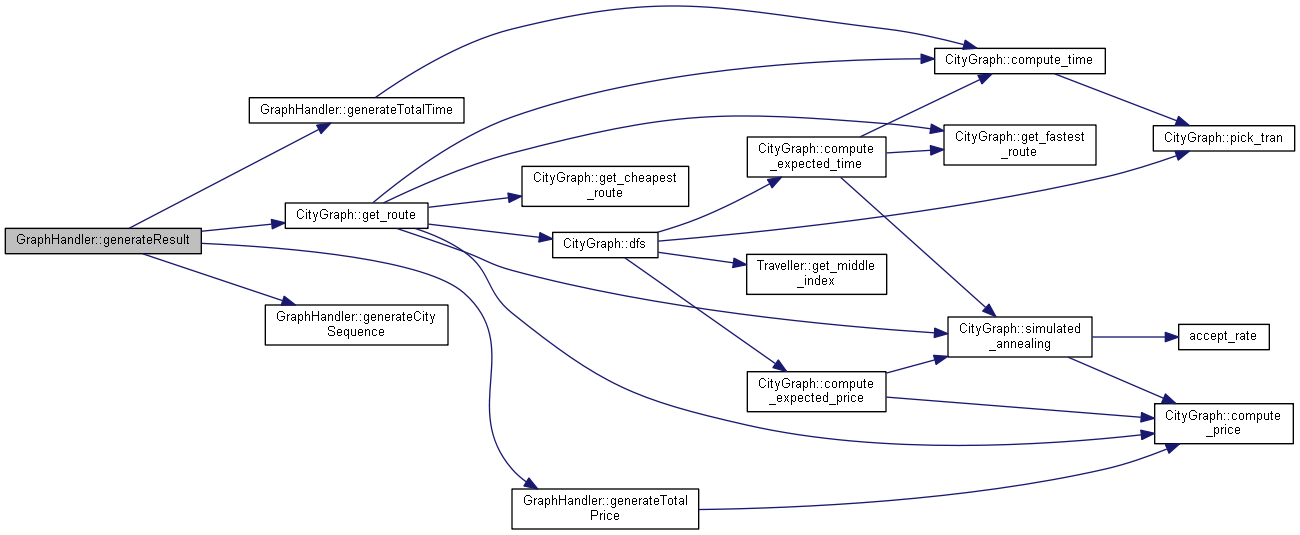
\includegraphics[width=1\textwidth]{graph_handler_generateResult.png}
 	\caption{GraphHandler::generateResult}
 	\label{genR}
 \end{figure}

主体部分的图形界面使用 Qt 实现,通过对 QML 的使用,我们很好地将前后端进行了分离,两者之间仅通过中间层以及信号和槽的方式进行必要的交互。

\chapter{算法实现}

\section{价格最低策略}

在我们的假设内,当不存在必须经过的中间城市时,该问题简化为单源最短路径问题,该问题最常见的解法为 \textbf{Dijkstra} 算法,其复杂度为 $O(|V|^2)$。我们在此处选择的算法为 \textbf{Floyd} 算法,其伪代码见算法~\ref{floyd}~,以此将全部点对之间的价格最低路径以及价格预先计算出来,并等待查询,该算法的时间复杂度为 $O(|V|^3)$。

\begin{algorithm}[H]
	\caption{\label{floyd}The Floyd Algorithm}
	\begin{algorithmic}[1]
		\Procedure{Floyd}{} 
		\State Let $dist$ be a $|V| \times |V|$ matrix of minimum distances initialized to $\infty$
		\For{\textbf{each} vertex $v$}
		\State $dist[v][v]\gets 0$
		\EndFor
		\For{\textbf{each} edge $(u,v)$}
		\State $dist[u][v]\gets w(u,v)$ \Comment the weight of the edge $(u,v)$
		\EndFor
		\For{$k$ \textbf{from} 1 \textbf{to} $|V|$}
		\For{$i$ \textbf{from} 1 \textbf{to} $|V|$}
		\For{$j$ \textbf{from} 1 \textbf{to} $|V|$}
		\If{$dist[i][j] > dist[i][k] + dist[k][j]$}
		\State $dist[i][j] \gets dist[i][k] + dist[k][j]$
		\Comment also update our route here
		\EndIf
		\EndFor
		\EndFor
		\EndFor
		\EndProcedure
	\end{algorithmic}
\end{algorithm}

当存在中间城市时,我们可以把``源城市-中间城市、中间城市-目标城市''的最短路径作为``源城市-中间城市-目标城市''的最短路径。此时中间城市的排序就成为了关键问题,该问题与旅行商问题比较类似。我们使用广为人知的模拟退火算法来处理此问题,模拟退火算法的一般流程见算法~\ref{sa}~。对于该问题,\textbf{ENERGY} 函数就是随机生成的路径序列可以达到的最低价格,而我们使用的\textbf{ACCEPT}函数的定义如下:
\begin{lstlisting}[language=C++]
static inline double accept_rate(const int &new_energy, const int &old_energy, const double &temperature) {
	return old_energy > new_energy ? exp((old_energy - new_energy) / temperature) : 1.0f;
}
\end{lstlisting}
后续的时间最短策略使用的算法也是模拟退火算法,唯一修改的只有\textbf{ENERGY},恕不再进行详细说明。

\begin{algorithm}[H]
	\caption{\label{sa}The Simulated Annealing Algorithm}
\begin{algorithmic}[1]
	\Procedure{SimulatedAnnealing}{}
	\State $T\gets T_{max}$
	\State $best\gets$ \textbf{\Call{INIT}{$ $}}
	
	\While{$T>T_{min}$}
	\State $next\gets $ \textbf{\Call{NEIGHBOUR}{$T, best$}}
	\State $\Delta E\gets$ \textbf{\Call{ENERGY}{$next$}} $-$ \textbf{\Call{ENERGY}{$best$}}
	\If{$\Delta E < 0$}
	\State $best\gets next$
	\ElsIf{\Call{random}{$ $} $<$ \textbf{\Call{ACCEPT}{$T,\Delta E$}}}
	\State $best\gets next$
	\EndIf
	\State $T\gets$ \textbf{\Call{COOLING}{$T,best$}}
	\EndWhile \\
	\Return $best$
	\EndProcedure
\end{algorithmic}
\end{algorithm}

\section{时间最短策略}

在时间最短策略下寻找最优策略的思路于上一策略一致,都是使用\textbf{预处理 + 模拟退火}的方式实现快速求解。两者的不同就是在时间最短策略中,时间这一维度产生了重要的影响,也就是说,鲈形者的离开时间左右了算法的结果。不过好在一天只有二十四个小时,因此对于每一对城市每到整点时刻的最优结果记录一下即可。在这里,为了体现出于上一个策略的不同,我们使用了平均时间复杂度为 $O(e)$ 的 SPFA\footnote{段凡丁.关于最短路径的SPFA快速算法[J].西南交通大学学报,1994(02):207-212.}算法进行求解。其伪代码见算法~\ref{SPFA}~。

\begin{algorithm}[H]
	\caption{\label{SPFA}The SPFA Algorithm}
	\begin{algorithmic}[1]
		\Procedure{Spfa}{}
		\State Let $s$ be the source of the graph, $Q$ be a queue
		\For{\textbf{each} vertex $v$}
		\State $d[v] \gets +\infty$
		\State $flag[v] \gets false$
		\EndFor
		\State $d[s] \gets 0$
		\State $Q \gets {s}$
		\State $flag[s] \gets true$
		\While{ $Q \neq \Phi$ }
		\State $ u \gets Q.deque() $
		\State $flag[u] \gets false$
		\For{\textbf{each} vertex $v \in adj(u)$}
		\If{$d[v] > d[u] + \omega(u,v)$}
		\State $d[v] > d[u] + \omega(u,v)$
		\If{$flag[v] = false$}
		\State $Q.enqueue(v)$
		\State $flag[v] \gets true$
		\EndIf
		\EndIf
		\EndFor
		\EndWhile
		\EndProcedure
	\end{algorithmic}
\end{algorithm}

在对松弛的条件进行修改后,我们即可将之应用在我们的数据集上。最后使用模拟退火算法求解最优的中间城市次序即可。

\section{带时限的价格最低策略}
此时时间的限制对我们算法的策略选择有了很大关系,当时限很宽松时,旅行者大可选择最便宜的出行策略。但是当时限较为紧张时,旅行者就需要在各种情况下做出取舍,其结果很可能是杂乱无章的。此时如果继续使用模拟退火,其结果难以保证,甚至会产生又贵又慢的滑稽结果。因此,在这里我们选择了比较传统的 \textbf{DFS} 算法进行求解。

但是对于普通的 DFS 而言,我们的数据太过庞大(31 个城市, 5K+ 条线路),难以在可以接受的时间内得到结果。因此,为了减少运行时间,我们将 DFS 修改为 \textbf{有界深度优先搜索} 算法,同时使用启发式策略进行减枝处理。最终可以实现在 0.1 - 30 秒内得到较好的解。

\chapter{图形界面}

图形界面部分使用 Qt 的 QML 进行实现。QML 是一种多范式语言,其能使对象能够根据其属性以及如何关联和响应其他对象的更改来定义对象。与纯粹的命令式代码不同,属性和行为的变化通过一系列逐步处理的语句表达。QML 的声明性语法将属性和行为更改直接集成到单个对象的定义中,这些属性定义可以包含必要的代码,在情况复杂的自定义应用程序行为是必要的。其语法类似 CSS,适用于描述复杂的界面关系,辅以 C++ 可以快速实现出界面好看的应用程序。

该软件的界面风格来源于\href{https://www.google.com/design/spec/material-design/introduction.html}{Google Material Design Guidelines},见图~\ref{gui}~。共分为两大部分,左侧为完整的可以任意缩放的地图\footnote{数据来自\href{https://www.openstreetmap.org}{OpenStreetMap},在此表示衷心的感谢},规划后的路径会以红线的形式显示在地图上面;右侧是控制部分,用户的输入以及日志的输出都在这里进行。为了优化触屏用户的体验,控制栏尽可能地减少了用户自己输入的部分,只有日期、离开时间以及时限需要自己手动输入,其余部分仅需要滑动以及点选既可。

\begin{figure}[!htbp]
	\centering
	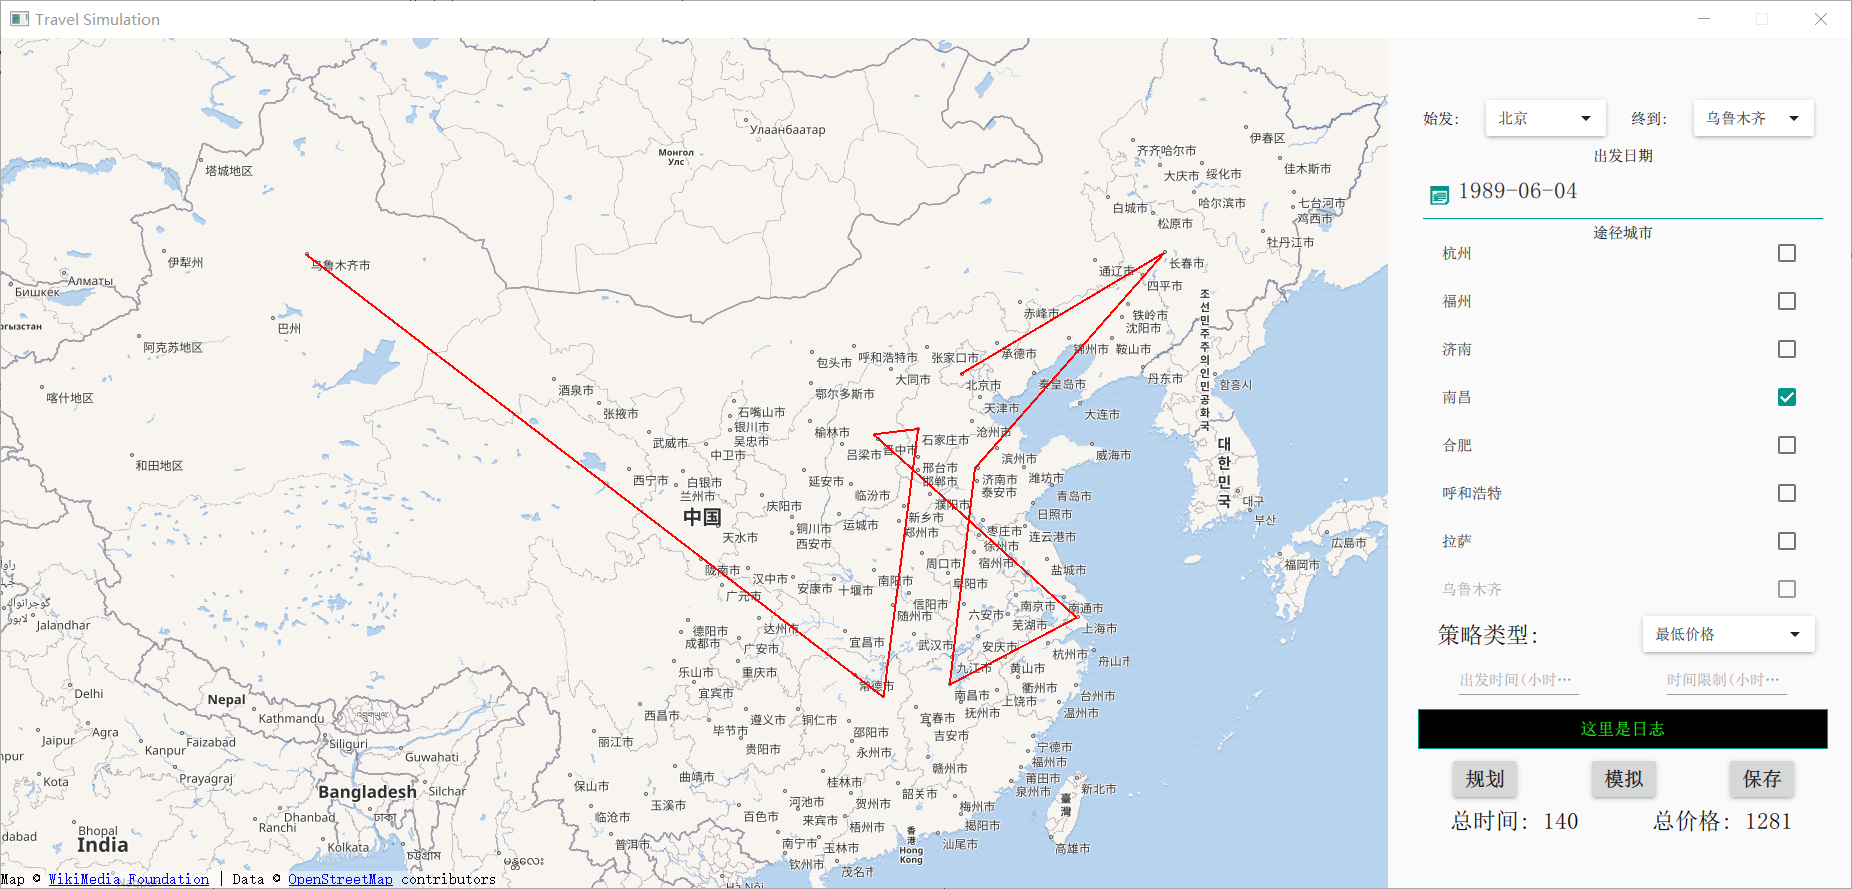
\includegraphics[width=1\textwidth]{gui.png}
	\caption{主体部分的包含关系}
	\label{gui}
\end{figure}

\chapter{爬虫部分}
该系统的爬虫部分主要采用 Python 的 requests 库实现,辅以代理池等技术保证不被网站的反爬虫技术限制。最终在 12306 上爬取到车票信息 14655 条,在携程网上爬取机票信息 930 条。该部分的源码现已开源,网址为 \href{https://github.com/kuso-kodo/kuso\_12306}{https://github.com/kuso-kodo/kuso\_12306}。

\section{火车票信息}
火车票的全部信息来自于铁总的 \href{https://www.12306.cn}{12306}。该部分代码位于 \href{https://github.com/kuso-kodo/kuso_12306/blob/master/src_12306/fetch.py}{fetch.py}。

12306 查询火车票的网址结构如下:
\begin{center}
	\begin{tabular}{cc}
		\hline
		\makebox[0.5\textwidth][c]{参数}	&  \makebox[0.2\textwidth][c]{含义} \\ \hline
		https://kyfw.12306.cn/otn/leftTicket/query & 查询网址 \\
		leftTicketDTO.train\_date & 要查询的日期 \\
		leftTicketDTO.from\_station & 始发站 \\
		leftTicketDTO.to\_station & 终点站 \\
		purpose\_codes & 乘客类型 \\ \hline
	\end{tabular}
\end{center}
需要注意的是站点需要使用内部电码来表示,获取内部电码的方式是访问 \href{https://kyfw.12306.cn/otn/resources/js/framework/station\_name.js}{https://kyfw.12306.cn/otn/resources/js/framework/station\_name.js} 获取形如``@bjb|北京北|VAP|beijingbei|bjb|0''的信息之后通过正则表达式获取所需信息。
访问该 API 返回的结果为 JSON,结果内包含了查询日期内全部车次的信息。使用恰当的方式提取即可。返回结果示例如下:
\begin{lstlisting}[language={}]
{"data":{"flag":"1","map":{"BJP":"北京","SHH":"上海"},"result":["X2r16oP8IGH94iXTfaiBVftWDflhurjVyMtLApUAqGtb%UMWvDzNbAPvs2JJgtpCsG2y5VUJ2l5mC%0AbxIfI7x4izoLOx2%2FQrCgmSw0FTE0HJRw34xqltxHR6QvsJs8ZzcVyUtiZ6O57m%2Btt%2BS7QUfVl23M%0AYkqXZBJdFwX3qw33jZUkU0PLe%2FYfzcinUaZk6VpcbaHLuYoflN4kdE6Vk%2BPrYGpwqehRkGoTElzS%0A8naAdzOg1VyR8vffGyFCZ%2B4F9ZbIMrm0Hm1cVV%2BA2RsOgIps8IwLambwpZ76GgZZRZj0O6%2B0TkGY%0AG8DGrhYOPKg%3D|预订|240000D70500|D705|BJP|SHH|BJP|SHH|21:21|09:20|11:59|Y|R3ArWiqJWSrjfblWAofOiX3%2Bo5Q7Ud8vVMTg1pnCJxohcTRTmikvHJ7nmlo%3D|20190530|3|P4|01|04|0|0||||有|||有||有||有||||O0J0O0I0|OJOI|0|0|null"]},"httpstatus":200,"messages":"","status":true}
\end{lstlisting}

查询车票价格的 API 如下:
\begin{center}
	\begin{tabular}{cc}
		\hline
		\makebox[0.5\textwidth][c]{参数}	&  \makebox[0.2\textwidth][c]{含义} \\ \hline
		https://kyfw.12306.cn/otn/leftTicket/queryTicketPrice & 查询网址 \\
		train\_no & 火车编号 \\
		from\_station\_no & 起始站编号 \\
		to\_station\_no & 结束站 \\
		seat\_types & 火车类型 \\
		train\_date & 出行时间 \\ \hline
	\end{tabular}
\end{center}
需要注意的是,在访问该网站查询价格之前,需要以相同的参数访问 \href{	https://kyfw.12306.cn/otn/leftTicket/queryTicketPriceFL}{	https://kyfw.12306.cn/otn/leftTicket/queryTicketPriceFL} 一次才可以获得正确的结果,否则只能收到出错的信息。这里的大部分参数都可以在上一个 API 的回应中找到。该 API 的返回结果也是 JSON,示例如下:
\begin{lstlisting}[language={}]
{"data":{"9":"17480","A9":"¥1748.0","M":"¥933.0","O":"¥553.0","OT":[],"WZ":"¥553.0","train_no":"240000G1010K"},"httpstatus":200,"messages":"","status":true}
\end{lstlisting}
使用恰当的方式从中提取价格即可。

通过使用 Python 对以上过程编程,最终获取到了 31 个目标城市之间的直达列车信息共 14655 条。城市列表如下:
\begin{lstlisting}[language=Python]
	city_list = ['北京', '天津', '上海', '重庆', '石家庄',
	'太原', '呼和浩特', '郑州', '长沙', '武汉',
	'哈尔滨', '长春', '沈阳', '成都', '昆明',
	'贵阳', '拉萨', '乌鲁木齐', '西安', '兰州',
	'银川', '西宁', '广州', '南宁', '海口',
	'南京', '杭州', '福州', '济南', '南昌',
	'合肥']
\end{lstlisting}

\section{机票信息}
机票的信息来自于\href{https://www.ctrip.com/}{携程网}。该网站的爬取较为简单,故不再说明,只是在此记录下核心代码:
\begin{lstlisting}[language=Python]
def get_flight_prices(site_info, time_info):
	url = 'https://flights.ctrip.com/itinerary/api/12808/products'
	headers = {'referer': 'https://flights.ctrip.com/itinerary/oneway',
	'content-type': 'application/json'}
	data = {
	"flightWay": "Oneway",
	"classType": "ALL",
	"hasChild": False,
	"hasBaby": False,
	"searchIndex": 1,
	"airportParams": [{
	"dcity": site_info['depart']['city'],
	"acity": site_info['arrive']['city'],
	"dcityname": site_info['depart']['cityname'],
	"acityname": site_info['arrive']['cityname'],
	"date": time_info['date'],
	"dcityid": site_info['depart']['cityid'],
	"acityid": site_info['arrive']['cityid']
	}]
	}
	res = None
	while not res:
		res = get_resp(url, json.dumps(data), headers)
	if 200 <= res.status_code < 300:
		return parse(res.text)
	else:
		print('CTrip Sucks')
		return []
\end{lstlisting}

为了加快爬取速度以及防止被限制,我们在这里使用公开的 IP 代理信息搭建了代理池,最终在十分钟内爬取了 31 个城市间的飞机信息共 930 条。
\chapter{日志模块}

\chapter{测试与分析}

\chapter{总结}

\end{document}